\documentclass{article}

\usepackage[utf8]{inputenc}
\usepackage{setspace}
\usepackage[
	a4paper,
	total={17cm,25cm},
	top=3cm, left=2cm,
	includefoot
	]{geometry}
\usepackage[
	english,
	czech
	]{babel}
\usepackage[autostyle]{csquotes}
\usepackage{caption}
\usepackage{graphicx}
\graphicspath{{./assets/}}

\title{Návrh hry - Blokranč}
\author{Petr Maronek}
\date{5.11.2022}

% 	Vysvětlivky
%	\section* hvězdička znamená, že má LaTeX odebrat číslování

\begin{document}
	\begin{spacing}{1.15}
		\rmfamily
		\maketitle
		\begin{center}
			\textbf{Vysoká škola finanční a správní}\linebreak
			Fakulta právních a správních studií\linebreak
			Návrh počítačových her\linebreak
			Zimní semestr 2022\linebreak
			Vedoucí práce: \textbf{doc. Ing Stanislava Mildeová CSc.}
		\end{center}
		\pagebreak
			
		\section*{Abstrakt}
		Hra v prohlížeči na bázi těžby herních prostředků, která umožňuje hráči
        reálně zhodnocovat své majetky v herním prostředí. Pomocí herních tokenů
        může zdokonalovat své NFT nástroje, které těží více těchto tokenů.
        Tokeny a NFT se poté dají prodat na trhu za reálnou hodnotu.
				
		\section*{Klíčová slova}
		krypto, NFT, farma, playToEarn, prohlížeč
		\pagebreak
		    
		\section*{Úvod}
		Bloranč je hra postavená na \textit{blockchain} technologii. V zásadě se
        jedná o software, který ke svému fungování využívá principů na bázi
        ekonomiky spojené s tokeny, které mají svou tržní hodnotu. Hra bude
        plnit takzvaný model "Play To Earn" což se dá volně přeložit jako
        "Vydělej si hraním". Do těchto typů her je nicméně nutná počáteční
        investice reálných peněz na nákup tokenů potřebných k následnému nákupu 
        či vyrobení si nezbytných nástrojů k hraní hry. Na následujících
        stránkách popíši, jaký má taková hra potenciál z hlediska jiných
        aplikací jejího konceptu a také jak může demostrovat reálné chování se 
        uživatelů v neregulovaném, a do značné míry reálném, ekonomickém
        prostředí. Celkový návrh hry rozdělím do fází konceptu, technologie a
        implememtaci, kde nastíním různá výhody a úskalí, která budou mít na
        provoz takové hry signifikantní dopad. 
		
		\section*{Struktura hry}
		V této části práce se zaměřím na prvky hry, které budou hrát
        nejdůležitější roli. Níže zobrazuji tyto prvky formou myšlenkové mapy,
        kde značím stěžejní pilíře hry.
		
		\begin{center}
			\label{Myšlenková mapa}
			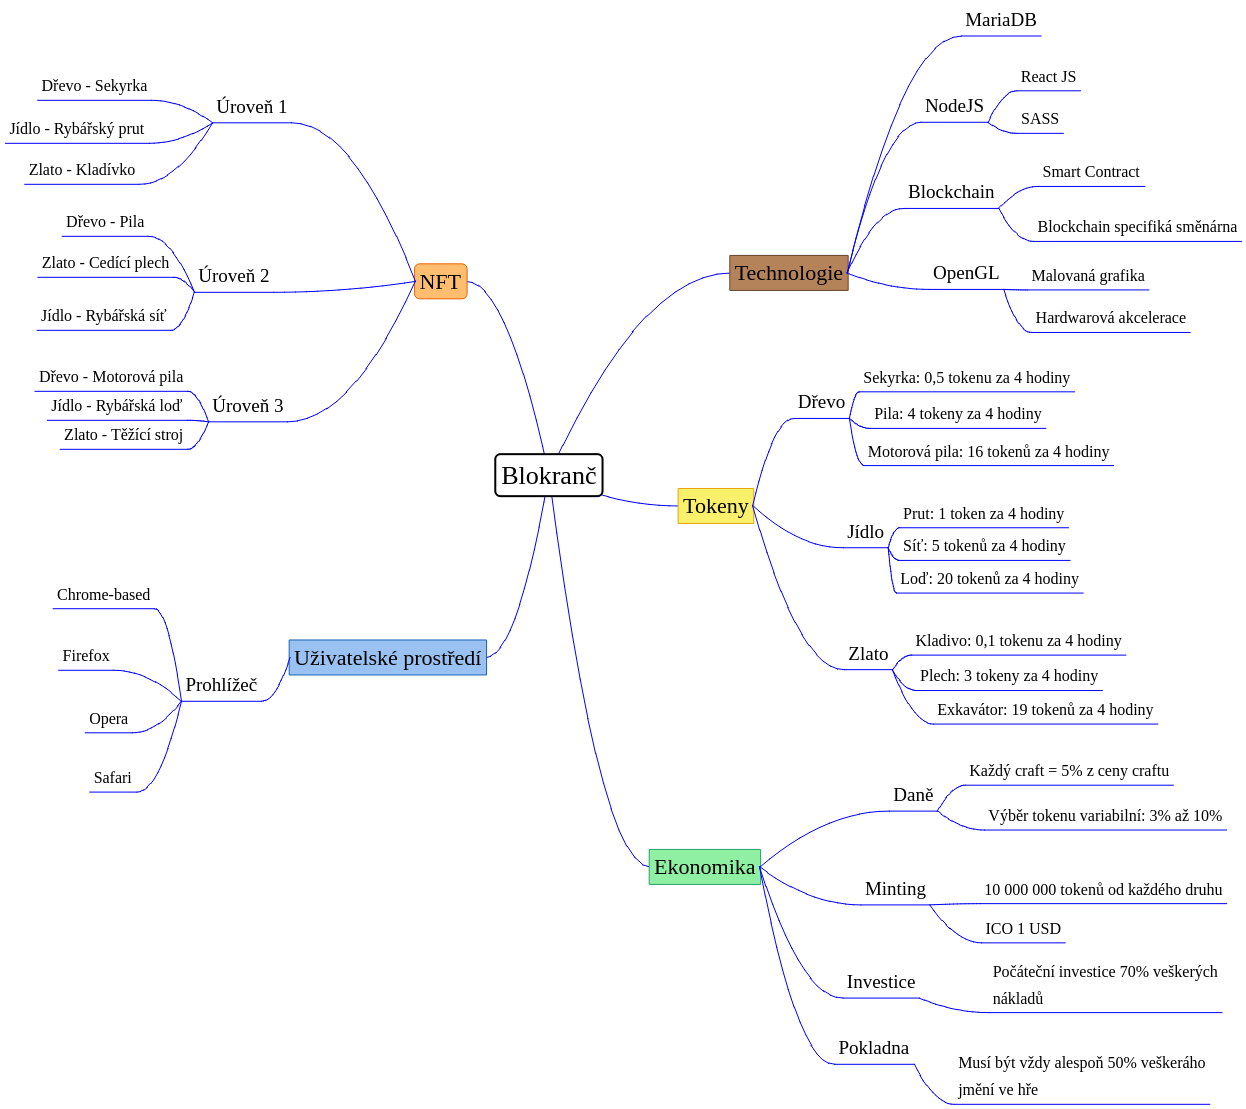
\includegraphics[scale=0.5]{221104-NPH-Blokranč.png}
			\captionof{figure}{Myšlenková mapa}
		\end{center}
		
		\section*{Herní prostředí}
        Uživatelské prostředí pro hru je koncipováno zcela v internetovém
        prohlížeči. Veškeré zobrazovací prvky budou responzivní a budou využívat
        moderní optimalizační technologie. Toto téma více rozvedu v části práce
        ohledně použitých technologií. Obecně bude hra podporovaná na většině
        moderních zařízení od stolních počítačů až po mobilní zařízení. Bude
        tedy platormě agnostická. Protože se jedná o hru v prohlížeči, není
        třeba instalovat žádný software. Hra bude pouze vyžadovat přihlášení
        platného uživatele a to pomocí peněženky kryptoměn.
        
        \section*{Technologie}
        Technologie blockchainu je moderní způsob převádění digitálního
        vlastnictví mezi dvěma stranami v kyberprostoru s možností kompletní
        transparentnosti transakce. Protože tato práce pojednává o hře, která
        tuto technologii pouze využívá, zaměřím se nyní pouze na její konkrétní
        aplikaci. 

        \section*{Vývoj postavy a progres hráče}
        Proces, jak může hráč ve hře postupovat dále, je pevně svázán s herními
        pomůcky ve formě NFT a tokenů, které hráč za dobu rhaní naakumoloval.
        Nyní nastíním, jak takový proces mlže vypadat v reálné aplikaci.

	\end{spacing}
\end{document}

